\section{Introduction}
\label{sec:introduction}

% state the learning objective
\paragraph{} 
The objective of this laboratory assignment is to study an RC circuit containing a voltage source V A , a current-controlled voltage source V C , a voltage-controlled current source I B and a capacitor C connected to different fixed value resistors R 1 , R 2 , R 3 , R 4 , R 5 , R 6 and R 7 , through a sinusoidal analysis using the following equation: $v_s (t) = V_s u(−t) + sin(2 \pi ft)u(t) $. 
The circuit
can be seen in Figure 1.
In Section 2, a theoretical introduction is made in order to contextualize all the main principles that sustain our analysis of the circuit. This circuit is carefully analysed following the equation already presented that describes our RC circuit. In Section 4, the circuit is analysed by simulation and the results are compared to the theoretical results obtained in Section 3. The conclusions of this study are outlined in the final part of the report, in Section 5.

\begin{figure}[h] \centering
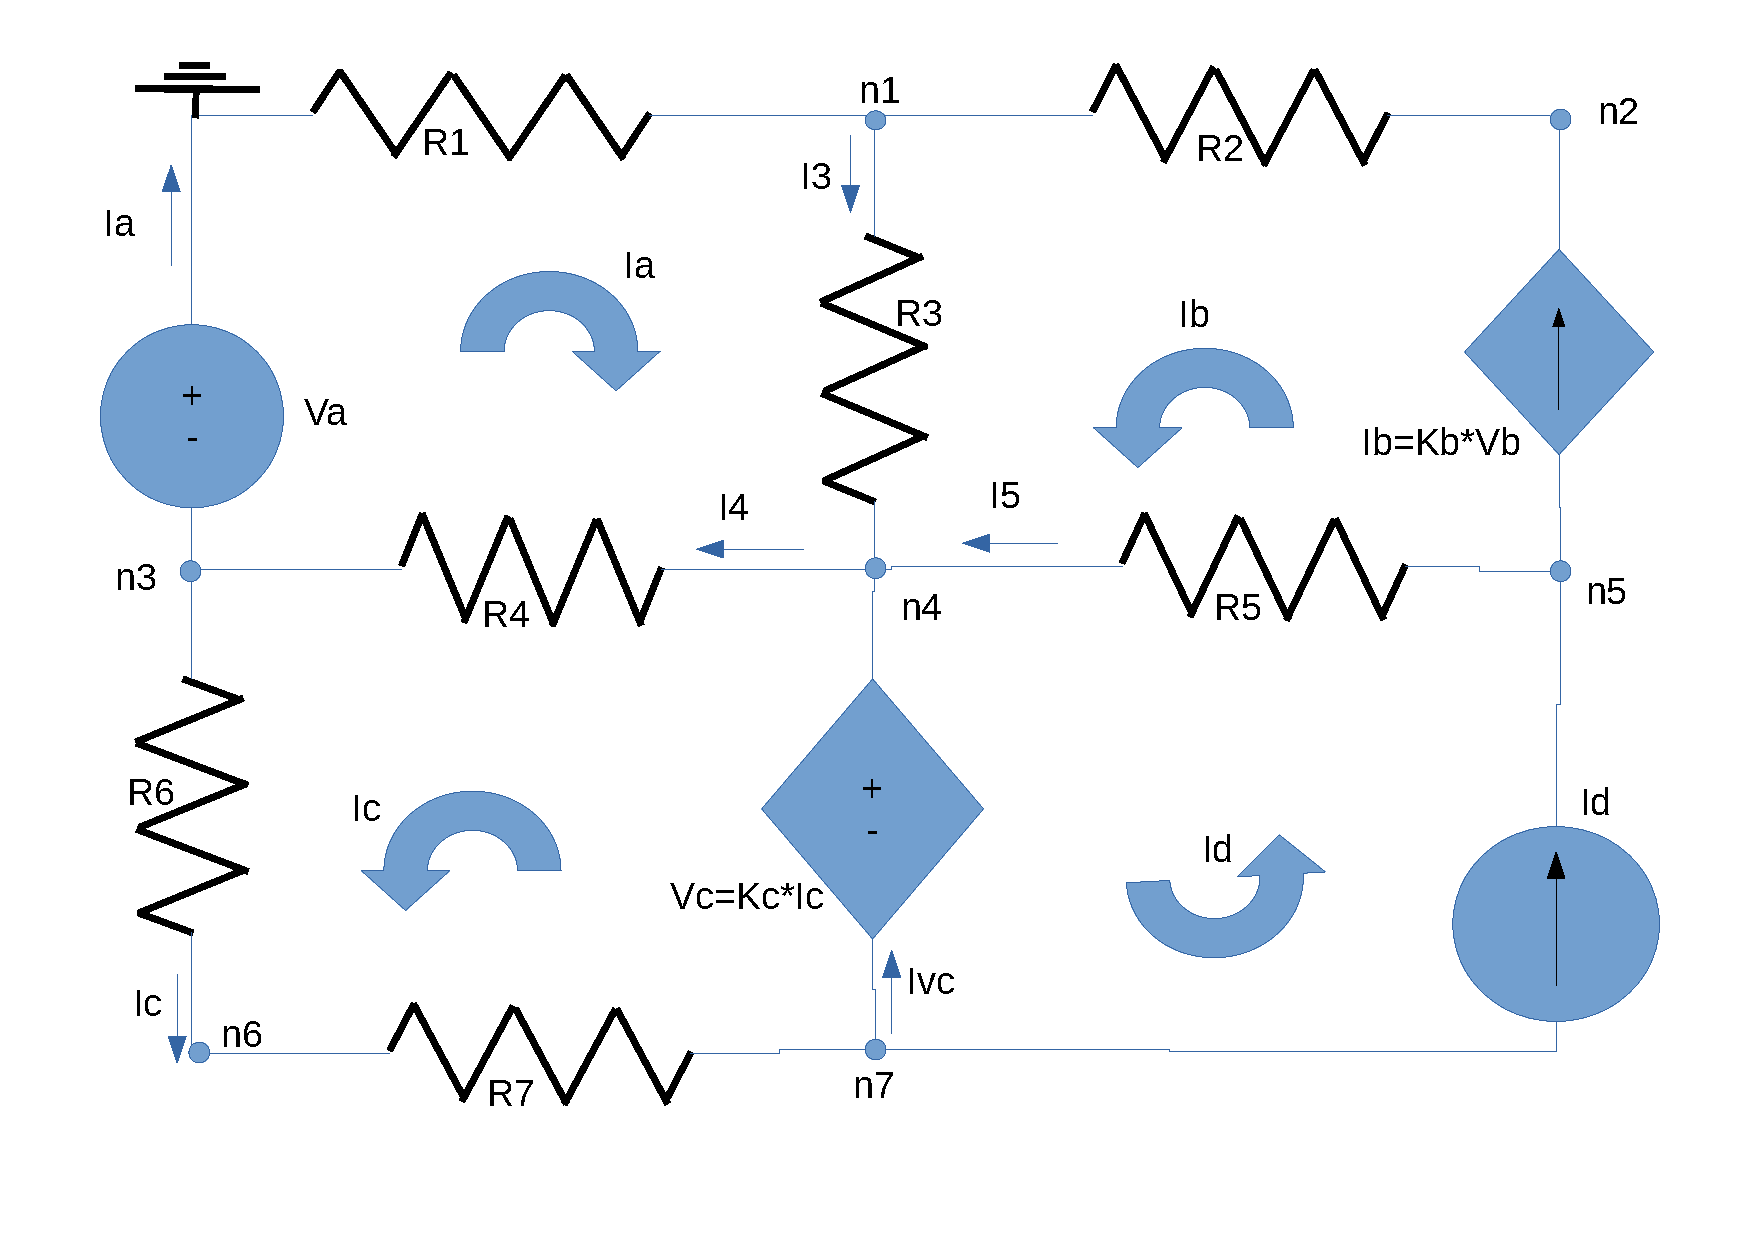
\includegraphics[width=0.4\linewidth]{circuit.pdf}
\caption{Second laboratory circuit.}
\label{fig:circuit}
\end{figure}

